\documentclass{beamer}
\usepackage{textcomp}
\usepackage{graphicx}
\title{Introduction to the FEMA database of RBI notifications}
\author{Gausia Shaikh}
\begin{document}
\begin{frame}
\maketitle
\end{frame}
\begin{frame}
\frametitle{Why create this database?}
\begin{itemize}
\item Questions
\begin{enumerate}
\item Does international discourse post the 2008 crisis account for interventions such as those imposed in India?
\item Do popular indices take into account such interventions?
\item Can specific interventions be studied to do an impact assessment?
\end{enumerate}
\item How will these be answered?
\begin{itemize}
\item Track amendments to FEMA Regulations and trends in foreign exchange policy;
\item Highlight how controls in India since 2008 are intrusive and discourage foreign investment;
\item Find events for impact assessment of capital controls as done with February 03, 2015 notification on long term FPI borrowings;
\item Challenge accuracy of the Chinn-Ito Index. See similar indices.
\end{itemize}
\end{itemize}
\end{frame}
\begin{frame}
\frametitle{Source of information}
RBI website \textrightarrow Foreign Exchange Management \textrightarrow Notifications
\begin{center}
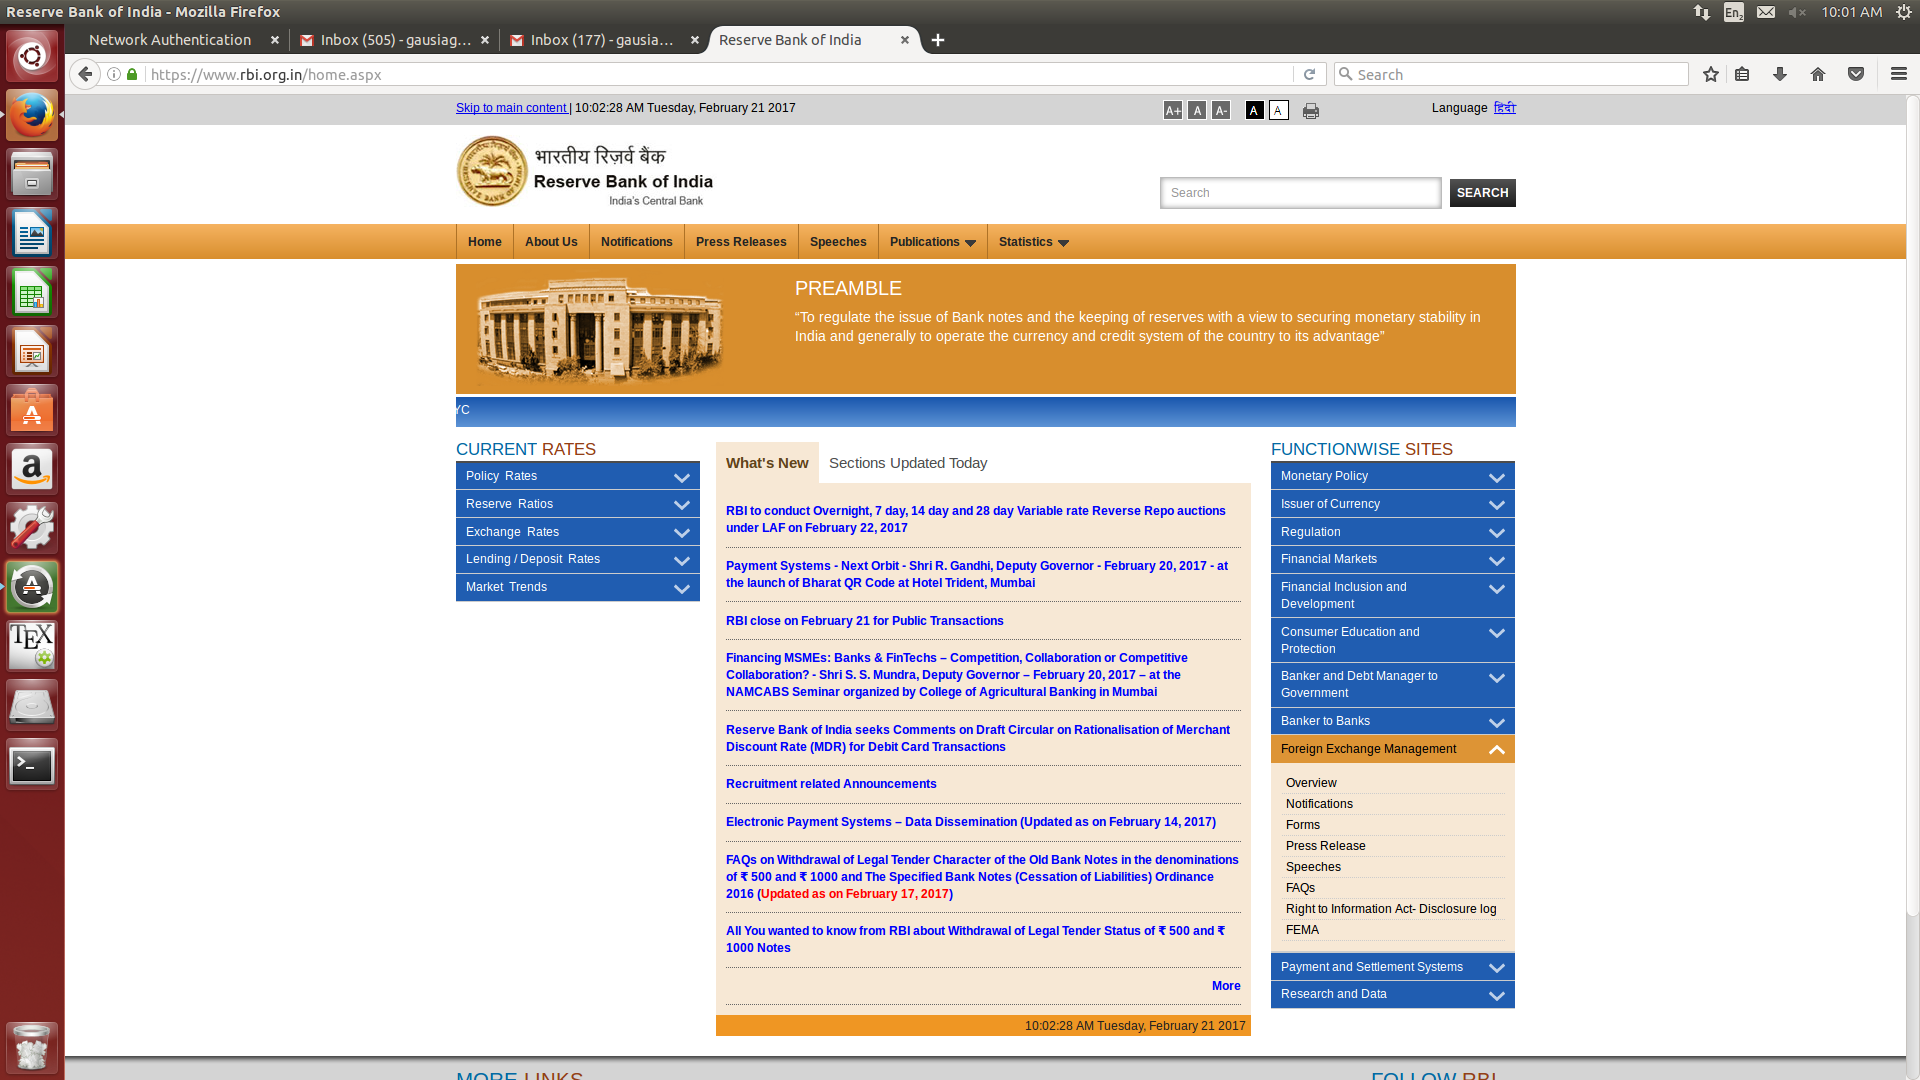
\includegraphics[height=65mm, width=95mm]{PICTURES/20170221_RBIHome.png}
\end{center}
\end{frame}
\begin{frame}
\frametitle{Source of information contd.}
Notifications \textrightarrow Year wise \textrightarrow Month wise
\begin{center}
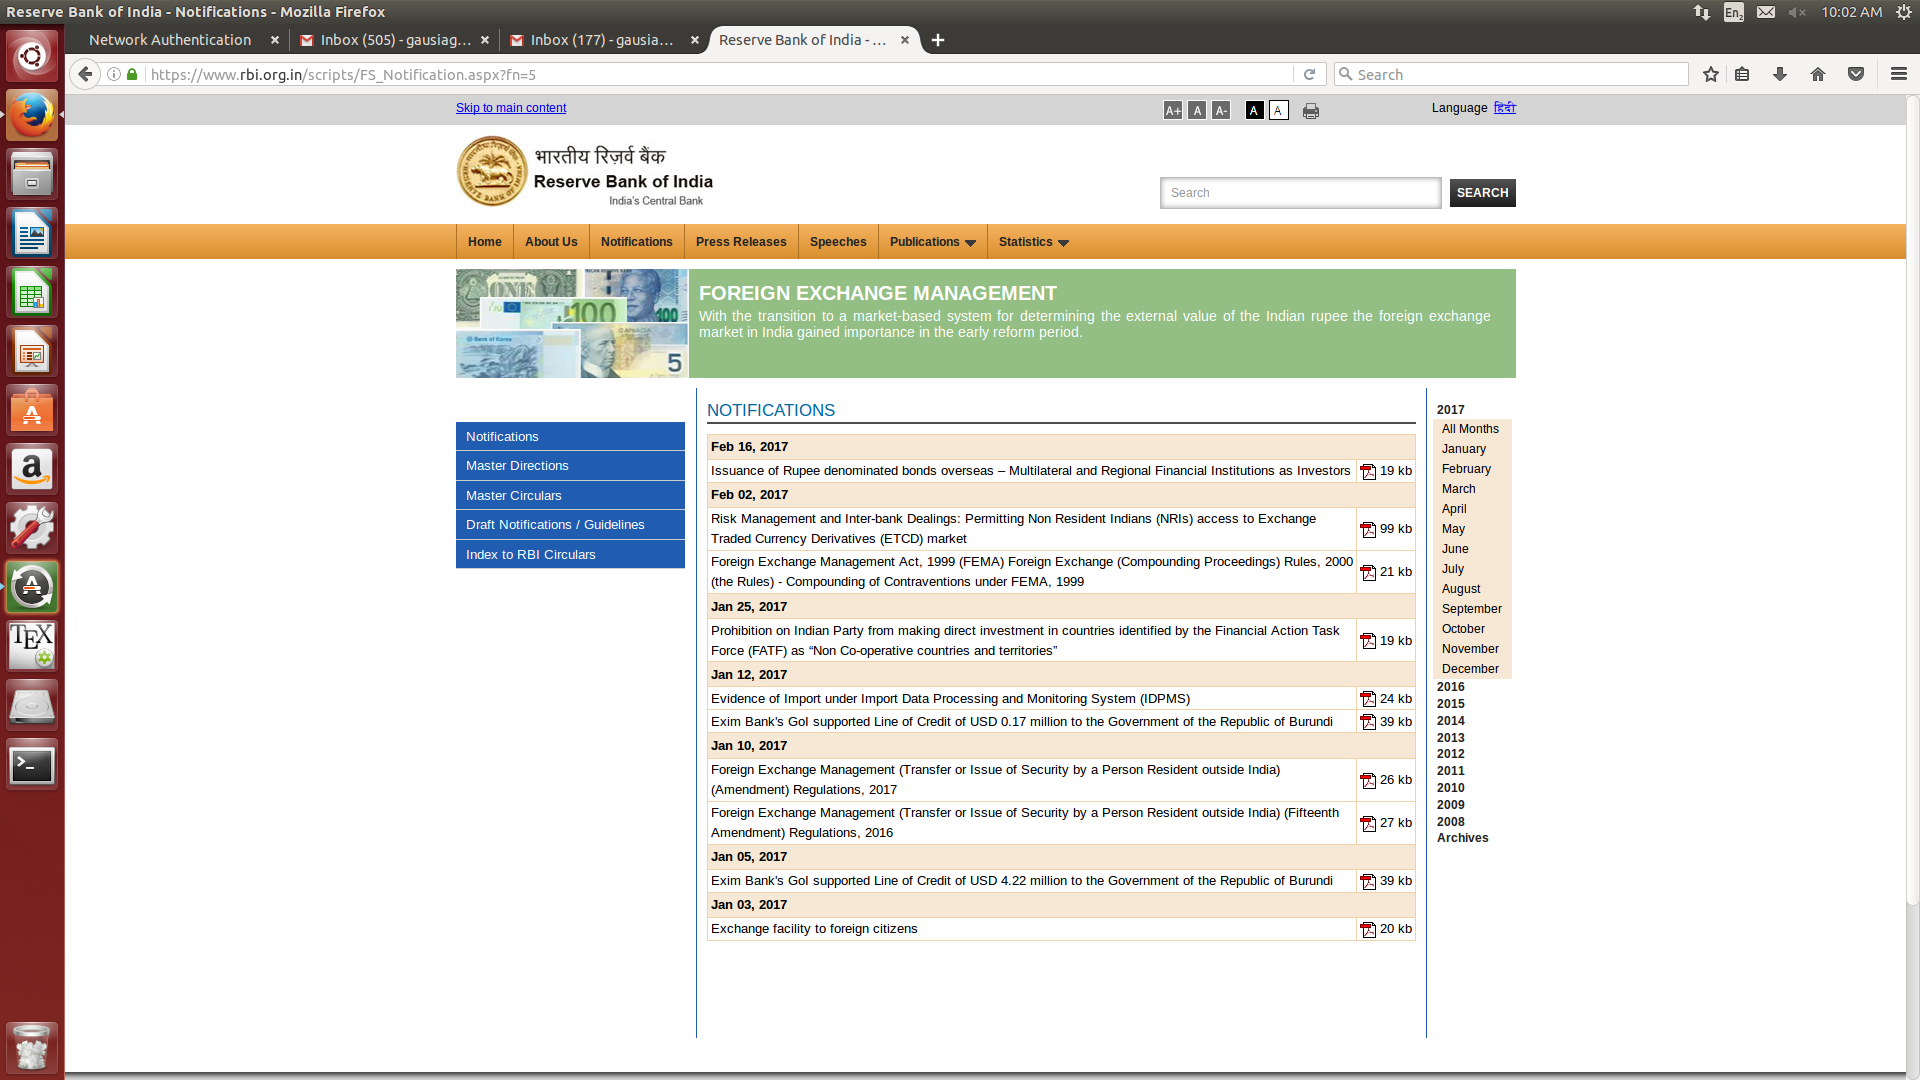
\includegraphics[height=65mm, width=95mm]{PICTURES/20170221_FEMANotifications.png}
\end{center}
\end{frame}
\begin{frame}
\frametitle{Form of notification}
\begin{center}
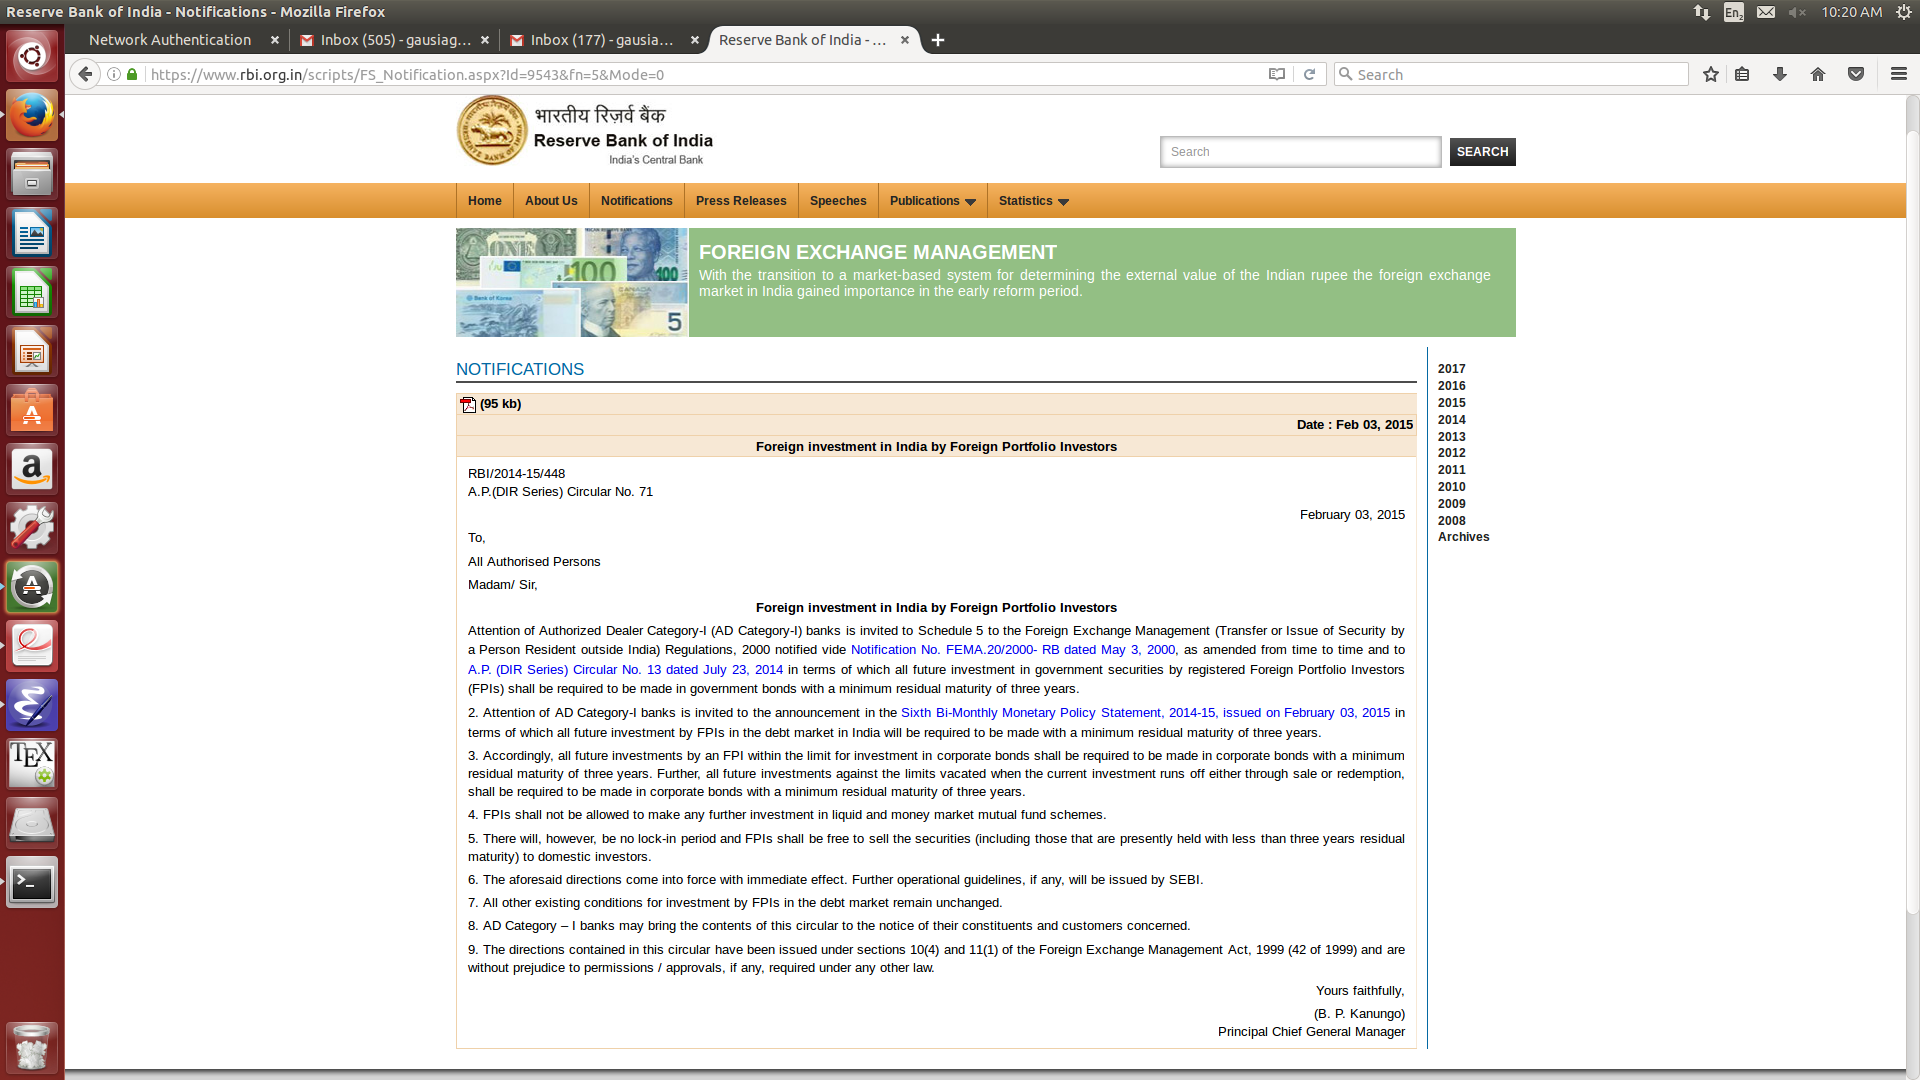
\includegraphics[height=80mm, width=95mm]{PICTURES/20170221_sampleNotification.png}
\end{center}
\end{frame}
\begin{frame}
\frametitle{Input fields}
\begin{enumerate}
\begin{tiny}
\item \textbf{Date of notification:} 03-02-2015
\item \textbf{Subject:} Foreign investment in India by Foreign Portfolio Investors
\item \textbf{Brief description:} All future investments by an FPI within the limit for investment in corporate bonds shall be required to be made in corporate bonds with a minimum residual maturity of three years.Further, all future investments against the limits vacated when the current investment runs off either through sale or redemption, shall be required to be made in corporate bonds with a minimum residual maturity of three years. 
\item \textbf{Target industry:} FPI
\item \textbf{Asset class:} Corporate Bonds
\item \textbf{Procedure / Intervention:} Intervention
\item \textbf{Limit changes:} Minimum residual maturity of 3 years
\item \textbf{Restricition / Liberalisation:} Restriction
\item \textbf{Score:} -1
\item \textbf{url:} \url{https://rbidocs.rbi.org.in/rdocs/notification/PDFs/71APDIR030215.pdf}
\end{tiny}
\end{enumerate}
\begin{tiny}
\emph{\textbf{1},\textbf{2} and \textbf{10} taken as is from the notification while \textbf{3 - 8} derived from reading of the notification.}
\end{tiny}
\end{frame}
\begin{frame}
\frametitle{Method of data compilation}
\begin{itemize}
\item Manually done
\item \emph{Is there any way to at least extract date, subject and url without human intervention?}
\end{itemize}
\end{frame}
\begin{frame}
\frametitle{Compilation so far}
\begin{itemize}
\item \textbf{Aimed timeline:} 2008 to 2017
\item Data is stored chronologically backwards
\item Data from 2013 to February 02, 2017 has been updated but with the following fields only: Date, Subject, Brief Decription and url
\end{itemize}
\end{frame} 
\begin{frame}
\begin{center}
Feedback and suggestions
\end{center}
\end{frame}
\begin{frame}
\begin{center}
Thank you
\end{center}
\end{frame}
\end{document}
